\subsection*{Présentation de la base \emph{keane}.}

Cette seconde base présente un échantillon d'hommes sur leur historiques éducatif et d'emploi. Cette base est composée de 12 723 observations et de 7 variables :  l'éducation en année \emph{educ}, la couleur de peau \emph{black}, le salaire (exprimé en log) avec la variable \emph{lwage}, le niveau d'expérience sur le marché du travail \emph{exper} et le statut professionnel \emph{status}.

\vspace*{0.3cm}

Ce travail consiste à interpréter les déterminants du statuts professionnels entre être à un étudiant (\emph{school}), être un travailleur (\emph{work}) et être ni l'un, ni l'autre (\emph{home}). Nous chercherons à expliquer le choix du statut par l'expérience (+ l'expérience au carré) et la couleur de peau.


%%%%%%%%%%%%%%%%%%%%%%%%%


\subsection{L'hypothèse : \emph{Independance of Irrelevant Alternatives} (IIA).}

Le modèle Logit conditionnel est construit sur l’hypothèse d’indépendance des alternatives non pertinente (Independance of Irrelevant Alternatives). L'IIA que la probabilité conditionnelle ne dépend pas des autres alternatives. En d'autres termes, le rapport de probabilités entre deux modalités est indépendant des autres modalités de la variable d’intérêts. Le corolaire de cette propriété est : ajouter une modalité ou bien en supprimer une ne modifie par les rapports de probabilités. 

\vspace*{0.3cm}

Dans notre cas, nous travaillons sur le statut professionnel, variable qui prendre trois modalités : \emph{school}, \emph{home} et \emph{work}. Pour estimmer la probabilité de chaque modalité, nous utilisons la formule suivante : 

\begin{align*}
    p_i = P(y_i = j \: | \: X_i = x_i) = \frac{e^{x_{ij} \cdot \beta_j}}{\sum_{j=1}^{K} e^{x_{ij} \cdot \beta_j}} 
\end{align*}

Nous allons rajouter une nouvelle catégorie : \emph{unemployment} et nous estimons à nouveau le modèle avec cette nouvelle catégorie. Nous notons les probabilités associées aux modalités respectivement $p_{work}$, $p_{home}$, $p_{school}$ et $p_{unemployment}$. L'hypothèse $IIA$ est acceptée si l'ensemble des rapports des différents probabilités ne se modifie pas entre la période 1 (3 modalités) et la période 2 (4 modalités). Économétriquement, nous posons les hypothèses suivantes : 

\begin{equation*}
	\left\lbrace
		\begin{aligned}
            H_0 :& \left( {\frac{p_{home}}{p_{school}}} \right)_1 = \left( {\frac{p_{home}}{p_{school}}} \right)_2 \: et \: \: \left( {\frac{p_{home}}{p_{work}}} \right)_1 = \left({\frac{p_{home}}{p_{work}}} \right)_2 \: et \: \: \left({\frac{p_{work}}{p_{school}}}\right)_1 = \left({\frac{p_{work}}{p_{school}}}\right)_2 \\ 
            H_1 :& \: la \: condition \: n \: est \: pas  \: vérifiée
		\end{aligned}
	\right.
\end{equation*}

Pour tester cette hypothèse, nous procédons aux tests \emph{Hausman et Mac Fadden} et celui de \emph{Small-Hsiao} (qui est plus robuste que le premier). La statistique du test est comparée à la valeur critique de la table du $\chi^2$ à $K$ degrés de liberté (avec $K$ le nombre de composante du vecteur $\beta_c$ dans le test de Hausman \footnote{Le test d'Hausman correspond à la statistique : $H = (\beta - \beta_c)^T \cdot V(\beta)-V(\beta_c)) ^{-1} \cdot (\beta - \beta_c) \backsim \chi^2 \: sous \: H_0$}). Si la statistique du test est supérieure à la valeur critique alors, l'hypothèse nulle $H_0 : IIA$ est rejetée. 


\subsection{Estimation d'un Logit multinomial.}

Avant de commencer à interpréter à la table de résultats, nous testons la validité du modèle et plus particulièrement l’hypothèse $IIA$. Nous disposons de plusieurs de tests dont deux de \emph{Hausman} et le test de \emph{Small-Hsiao}. Le test de Hausman rejette l’hypothèse nulle $H_0 : IIA$ au seuil de 5\%. Le test de Small Hsiao, plus robuste, ne rejette pas l’hypothèse nulle. Le modèle est alors valide en s’appuyant sur ce test.
Nous obtenons la table de résultat suivante : 

\begin{figure*}[h]
    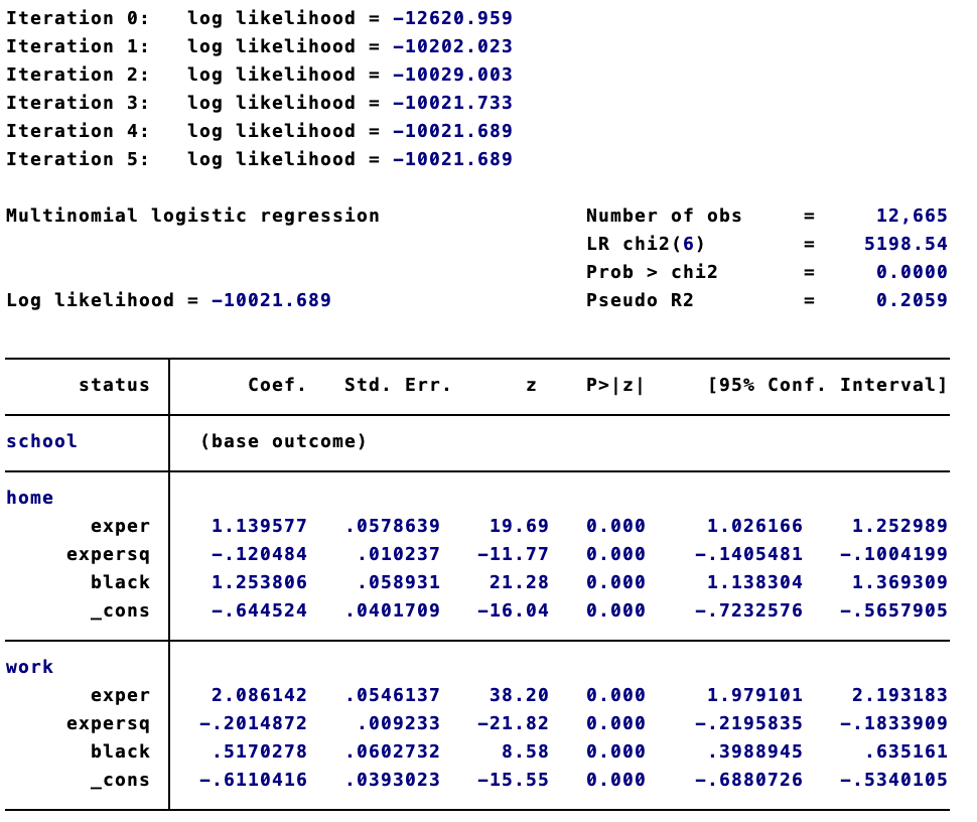
\includegraphics[scale = 0.55]{100_tab_results/mlogit.png}
    \centering
    % \label{fig:ProbaEntre0et1}
\end{figure*}

Avec l’estimation de ce modèle, nous avons perdu des observations : la base comprenait 12 723 observations et en compte désormais 12 665 (il manque au moins une valeur dans les variables pour cette observations). Néanmoins, la taille de l’échantillon reste important. 

\vspace*{0.3cm}

Ce modèle multinomial est estimé à l’aide de la méthode du maximum de vraisemblance. Il est globalement significatif (la $p_{value}$ du modèle est inférieur au seuil de 5\%). De plus, ce modèle dispose d’un pouvoir explicatif satisfaisant (le Pseudo $R^2$ est supérieur à 20\%).

\vspace*{0.3cm}

La modalité de référence de ce modèle est être à l’école (\emph{outcome 3}). L’ensemble des coeffients pour les trois variables sont significativement différent de 0. Nous ne pouvons pas interpréter davantage, les coefficients sont construits sur deux élements non séparément identifiés. Nous pourrons interpréter les résultats grâce aux rapports des risques relatifs. 

\subsection{Les rapports des risques relatifs du Logit multinomial.}

L'estimation du Logit multinomial en mettant en évidence les Rapports des Risques Relatives (RRR), nous donne la table de résultat suivante : 

\begin{figure*}[h]
    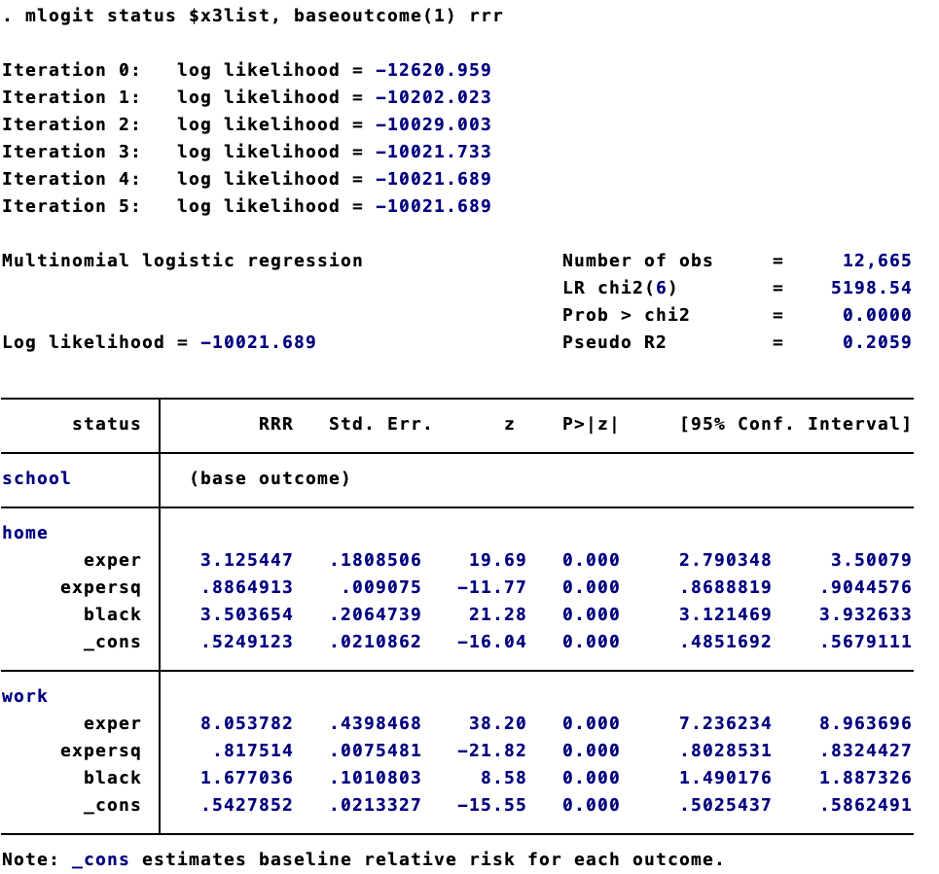
\includegraphics[scale = 0.55]{100_tab_results/mlogitRRR.png}
    \centering
    % \label{fig:ProbaEntre0et1}
\end{figure*}

Nous allons directement interpréter les résultats (les autres remarques sur la qualité du modèle ont été présenté dans la question précédente. Tous les coefficients sont significatifs et donc interprétables.

\vspace*{0.3cm}

Lorsque le niveau d’expérience augmente d’une année, alors il y a 3,12 fois plus (ou 212\% de plus) de chance d’être à la maison plutôt que d’être en cours toute chose égale par ailleurs. Il y a plus de 8 fois plus de chance de se trouver au travail plutôt qu’à l’école, lorsque le niveau d’expérience augmente d’une année. 

\vspace*{0.3cm}

Le RRR associé à la variable expérience au carré est inférieur à 1 et indique donc une relation négative, mettant en évidence alors une relation non constante et négative de la variable expérience (elle admet un maximum). En d’autres termes, il y existe un niveau d’expérience à partir duquel, une année d’expérience supplémentaire accroit la chance d’appartenir à la catégorie maison ou travail par rapport à l’école mais mois que les années d’année d’expérience précédente. Nous pouvons remarquer que le RRR associé à la catégorie maison est supérieur à celui du travail (toujours par rapport à la catégorie de référence). 

\vspace*{0.3cm}

Le RRR de la variable \emph{black} indique qu’il y a 3,5 fois plus (250\% de plus) de chance d’être à la maison plutôt que d’être à l’école quand nous sommes de couleur noir par rapport être blanc. Il y a 1,67 fois plus de chance d’être au travail plutôt qu’à l’école quand nous sommes noirs plutôt que blanc.



\subsection{Expérience et être noir : l'effet sur le statut.}

Ayant mis l’expérience dans le modèle et la couleur de peau, l’ajout de cette variable va permettre de capter un effet spécifique. Graphiquement, nous avons \ref{fig:effetjoint}

\begin{figure}[h]
    \caption{Effet joint de la couleur de peau et de l'expérience.}
    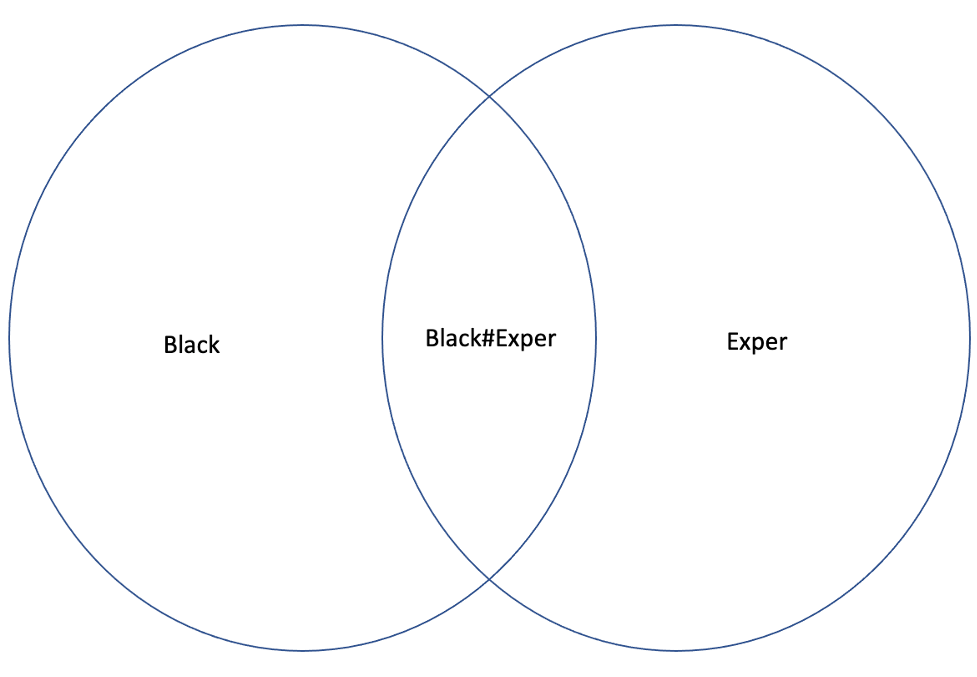
\includegraphics[scale = 0.5]{101_graphics/effetjoint.png}
    \centering
    \label{fig:effetjoint}
\end{figure}

La variable \emph{expérience} dans le modèle va capter l’effet de l’expérience (seul) et la variable \emph{black} va capter l’effet relatif à la couleur de peau (seul). La zone entre les deux cercles donne l’effet joint des deux variables. 

\vspace*{0.3cm}

Il existe de fortes inégalités aux États-Unis basé sur la couleur de peau à la fois sur le revenu, le patrimoine et le statut social. Nous allons donc pouvoir mesurer cette discrimination grâce à la variable d’interaction. Nous re-estimons le modèle en rajoutant cette variable. Nous obtenons la table qui suit : 

\begin{figure*}
    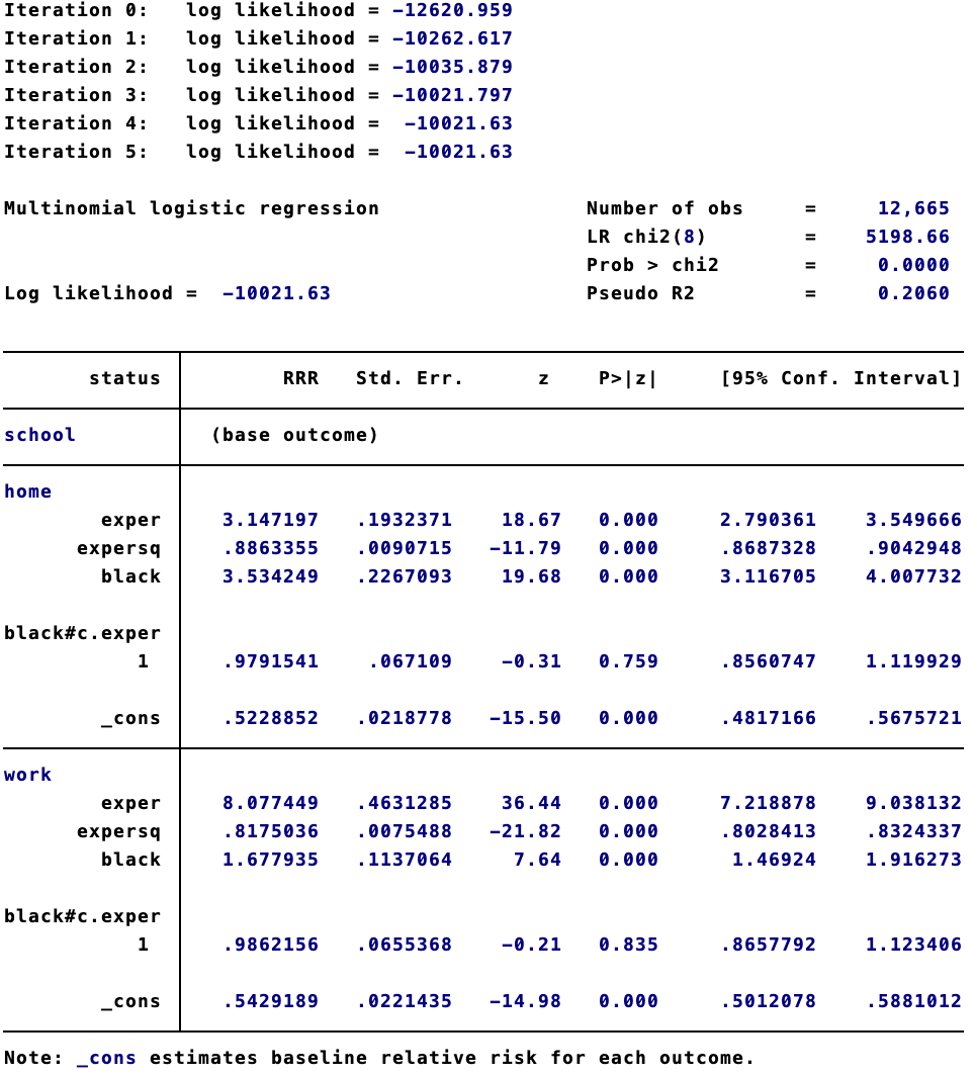
\includegraphics[scale = 0.55]{100_tab_results/mlogitRRRinteraction.png}
    \centering
    % \label{fig:ProbaEntre0et1}
\end{figure*}



Avant d’interpréter les coefficients, nous réalisons à nouveau le test $IIA$. Ici aussi, le test de Small-Hsiao indique l’hypothèse nulle d’IIA n’est pas rejetée. Le modèle est globalement significatif et le pseudo $R^2$ est satisfaisant (très légèrement supérieur à celui du précédent modèle. 

\vspace*{0.3cm}

La variable d’interaction n’apparait pas comme significativement différentes de 0 dans le cadre de ce modèle. Ce résultat apparait comme surprenant. Les RRR se sont vu modifié à la marge. 
Par ce modèle, nous ne pouvons pas assurer la mesure d’une discrimination ou du moins une particularité du l’expérience chez les personnes noires.



%%%%%%%%%%%%%%%%%%%%%%%%%%%%%%%%%%%%%%%%%%%%%%%%%%%%%%%%%%%%%%%%%%%%%%%%%%%%%%%

\subsection{Estimation par un modèle séquentiel.}

\subsubsection*{Pourquoi utiliser un modèle séquentiel ?}

Le modèle séquentiel permet de traiter une situation dans laquelle les modalités sont classés en parties. Ce modèle permet de découper les choix de décision en séquences, à chaque séquence, l’individu optimise son choix. L’avantage de ces modèles est de pouvoir relâcher l’hypothèse contrainte d’$IIA$. 


\subsubsection*{La construction de l'arbre.}

Dans notre cas, nous pouvons imaginer deux arbres séquentiels. Le premier traite les individus en fonction qu’ils soient actifs ou non (soit à l’école ou au travail ou bien à la maison). Le second arbre traite des individus qu’ils travaillent ou non (\emph{work} contre \emph{school} et \emph{home}). Nous allons modéliser le premier arbre \ref{fig:arbre} : 


\begin{figure}[h!]
    \caption{Arbre pour la construction du modèle Logit séquentiel.}
    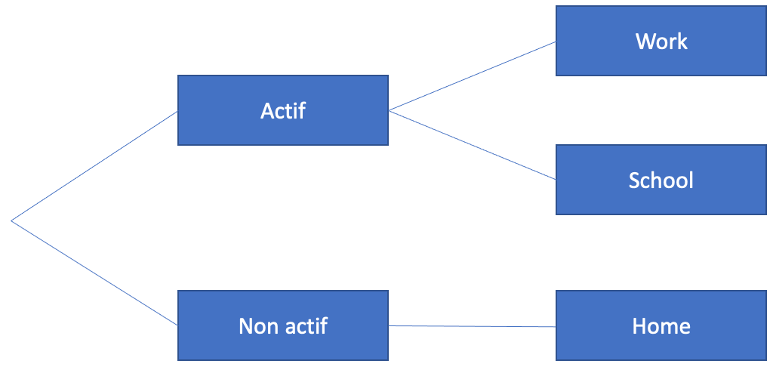
\includegraphics[scale = 0.7]{101_graphics/arbre.png}
    \centering
    \label{fig:arbre}
\end{figure}


\subsubsection*{Estimation et interprétation du modèle logit séquentiel.}

Nous obtenons la table de résultats suivante : 

\begin{figure*}[h]
    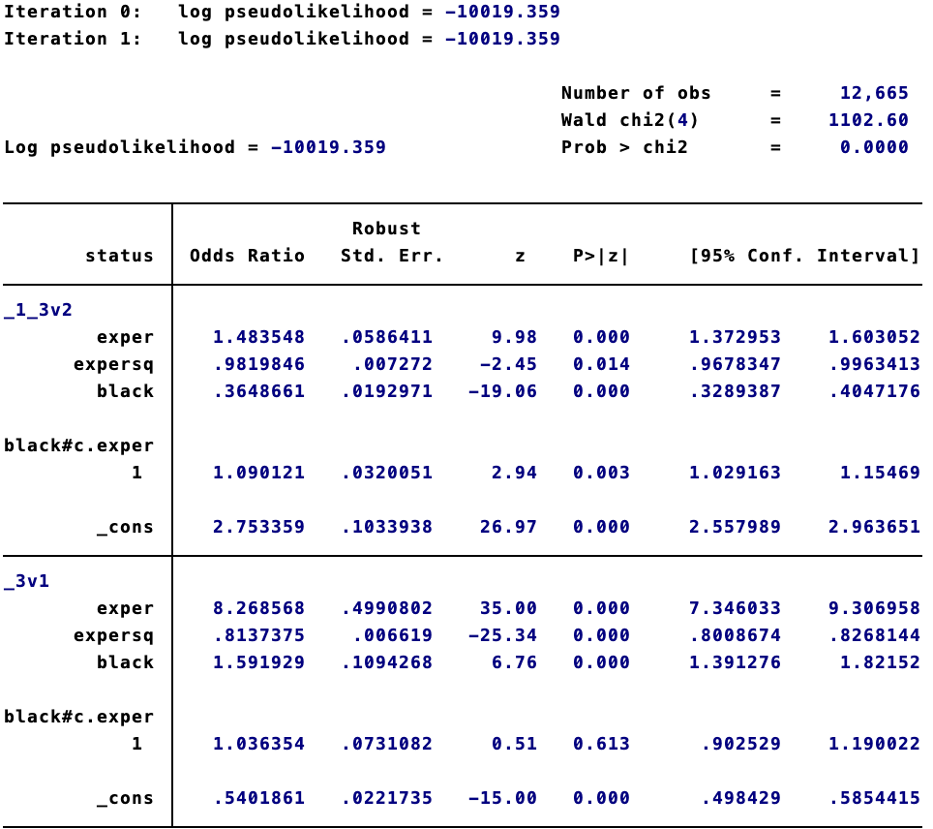
\includegraphics[scale = 0.55]{100_tab_results/logitsequentiel.png}
    \centering
    % \label{fig:ProbaEntre0et1}
\end{figure*}

Ce modèle est estimé par la méthode du maximum de vraisemblance. Comme pour le logit multinomial, le modèle ne considère pas l’ensemble de la population (perte d’observations du fait de valeurs manquantes). Le modèle est globalement significatif (la probabilité critique est inférieure à 5\%). Le modèle est estimé à l’aide des \emph{odd-ratio} pour faciliter l’interprétation.

\vspace*{0.3cm}

Nous obtenons deux tables : la première présente la possibilité de prendre le choix école ou bien travail au lieu de choisir être à la maison. Dans cette première régression, tous les Odd Ratio sont significatifs au seuil de 5\% (y compris la variable d’interaction). Choisir d’être actif par rapport à ne pas être actif augmente de 48\% lorsque nous avons une année d’expérience supplémentaire. La relation de l’expérience est là aussi inférieure à 1 indique une relation non linéaire qui admet un maximum. Être noir par rapport à être non noir augmente le risque de ne pas être actif de 63,52\% toutes choses égale par ailleurs. Enfin, le terme d’interaction est supérieur à 1. Nous pouvons alors l’interpréter, lorsque nous somme de couleur noir, si l’expérience augmente d’une année, la chance de choisir d’être actif par rapport à ne pas être actif augmente de 9\% toutes choses égale par ailleurs. 

\vspace*{0.3cm}

Dans la seconde table, nous comparons le fait de choisir le travail par rapport à l’école. Une année d’éducation supplémentaire augmente la chance d’être au travail de 726\% ($odd-ratio = 8,2$). La relation de l’expérience au carré est là aussi négative (inférieur à 1). Il existe donc bien un minimum. Être noir augmente la chance de travail de 59\% par rapport à choisir l’école. Le terme d’interaction n’est pas significativement différent de 0 dans cette table. Alors, il n’est pas possible d’interpréter le coefficient. 




